\chapter{Basics of Functions}
\section{Definition of a Function}

A \textbf{function} \(f\) from a set \(D\) to a set \(R\) is an assignment of exactly one element \(f(x) \in R\) to each element \(x \in D\).
if $f$ is a function from $D$ to $R$, we write\footnote{Sets and set builder notation are explained in more detail in \ref{ch:sets}.}
\[f:D \to R\]
and say that $f$ \emph{maps} $D$ to $R$.
\index{function}

  One technique that can help us understand functions is by describing them with words,
including mathematical language.
We can discuss the behavior of a function in general,
describing its properties, or we can discuss its behavior in more specific terms,
like when we evaluate a function at a certain value.

We can also talk about functions using visual language, as in graphs, arrow diagrams, and tables.
% There are, of course, many ways to visually represent a function, but for our purposes these will prove the most useful.
% This includes some numerical displays of functions, like with a table of values.
% We can consider tables to be a visual description of a function because they combines visual formatting with descriptive data to produce a figural representation of a function's properties.

We will find graphs, in conjunction with the respective mathematical language, to be the most cohesive way to represent functions.
We should therefore attempt to be able to graph our functions whenever we wish to achieve the best possible understanding of them.

We will combine these techniques in an effort to paint a complete picture of its behavior.

\section{Properties of Functions}


\subsection{Domain and Range}

The set \(D\) of all possible input values is called the \textbf{domain} of the function.
\index{domain}

The set of all values \(f(x)\) as \(x\) varies throughout \(D\) is called the \textbf{range} of the function, representing the output value of \(f\) at \(x\).
\index{range}

 The \textbf{natural domain} of a function is the largest set of real \(x\)-values for which a function returns real \(y\)-values.
A function is said to be \textbf{real-valued} when \(D = \mathbb{R}\).
That is, the domain is equal to to the set of real numbers.
This means that we can put an arbitrary real number into the function and it will return a real $y$-value.

 \begin{remark}
     When we define a funciton \(y=f(x)\) with a formula and the domain is not stated explicitly or restricted by context, the domain is assumed to be the \emph{natural domain}.
   \end{remark}
   \index{natural domain}

  The \textbf{vertical line test} for a function is based on the idea that if \(a\) is in the domain of the function \(f\) then the vertical line \(x=a\) will intersect the graph of \(f\) at a single point \( \big(a,f(a)\big)\).
  \index{vertical line test}

\begin{figure}[H]
  \begin{center}
    \subfigure[This passes the vertical line test]{
      
\includegraphics[width=0.4\textwidth]{continuous/functions/vlt1}
    }
    \subfigure[This fails the vertical line test]{
      
\includegraphics[width=0.4\textwidth]{continuous/functions/vlt2}
    }
  \end{center}
  \caption{Examples of the vertical line test.}
\end{figure}


\subsection{Dependent and Independent Variables}
  The letter \(x\) in the notation \(y=f(x)\) is called the \textbf{independent variable} of the function, representing the input value of \(f\).
  \index{independent variable}

  The letter \(y\) in the notation \(y=f(x)\) is called the \textbf{dependent variable}.
  It varies with respect to change in the dependent variable of the function.
  \index{dependent variable}

\subsection{Even and Odd Functions}

For a function $f$ in the form $y=f(x)$, we describe its type of symmetry by calling the function \textbf{even}\index{even functions} or \textbf{odd}\index{odd functions}.

An \textbf{even function} means $f(-x)=f(x)$.
An example of an even function is the function $f(x)=x^2$.
  \begin{figure}[H]
    \begin{center}
      \begin{tikzpicture}
        \begin{axis}[
            ylabel={\(f(x)=x^2\)},
            axis x line=bottom,
            axis y line=center,
            tick align=outside,
            yticklabels={,,}
            xticklabels={,,}
            xtickmax=10,
          ]
          \addplot[smooth,red]{x^2};
        \end{axis}
      \end{tikzpicture}
    \end{center}
    \caption{$f(x)=x^2$ is an \emph{even function}.}
  \end{figure}
  An \textbf{odd function} means $f(-x)=-f(x)$. An example of this is the function $f(x)=x^3$.
  \begin{figure}[H]
    \begin{center}
      \begin{tikzpicture}
        \begin{axis}[
            ylabel={\(f(x)=x^3\)},
            axis x line=bottom,
            axis y line=center,
            tick align=outside,
            yticklabels={,,}
            xticklabels={,,}
            xtickmax=10,
          ]
          \addplot[smooth,red]{x^3};
        \end{axis}
      \end{tikzpicture}
    \end{center}
    \caption{$f(x)=x^3$ is an \emph{odd function}.}
  \end{figure}
\subsection{Surjective, Injective, and Bijective Functions}

\begin{defn}
  \index{one-to-one}
  \index{injective}
  If each $f(x)$ value produced by a function $f$ can only be obtained by one unique $x$ value, then we say $f$ is \textbf{injective}, or \textbf{one-to-one}.

  \( f: D \to R \) is injective or one-to-one iff
  \[
    \forall{(x_1 \wedge x_2 \in D)}
    \big[f(x_1)=f(x_2)
    \to x_1=x_2\big].
  \]
  \begin{remark}
    This also means that for injective functions,
    \( x_1 \neq x_2 \to f(x_1) \neq f(x_2)\).
  \end{remark}
\end{defn}
\begin{figure}[H]
    \begin{center}
        \subfigure[The function \(f(x)=x^2\) is not \emph{one-to-one} because there are two possible \(x\)-values that can produce each given \(y\)-value.]
        {
          \begin{tikzpicture}
            \begin{axis}[
                ylabel={\(f(x)=x^2\)},
                axis x line=bottom,
                axis y line=center,
                tick align=outside,
                yticklabels={,,}
                xticklabels={,,}
                xtickmax=10,
              ]
              \addplot[smooth,red]{x^2};
            \end{axis}
          \end{tikzpicture}
        }
        \hspace{0.2in}%
        \subfigure[The function \(f(x)=x^3\) is \emph{one-to-one} because every given \(y\)-value is mapped from a unique \(x\)-value.]
        {
          \begin{tikzpicture}
            \begin{axis}[
                ylabel={\(f(x)=x^3\)},
                axis x line=bottom,
                axis y line=center,
                tick align=outside,
                yticklabels={,,}
                xticklabels={,,}
                xtickmax=10,
              ]
              \addplot[smooth,blue]{x^3};
            \end{axis}
          \end{tikzpicture}
        }
    \end{center}
  \end{figure}
  A function \(y=f(x)\) is one-to-one iff its graph intersects each horizontal line at most once.\index{horizontal line test}
\begin{defn}
  \index{onto}
  \index{surjective}
  \(f: D \to R \) is \textbf{surjective} or \textbf{onto} iff
    \[\forall (y \in R) \exists  (x \in D) \big[f(x)=y\big]. \]
\end{defn}
\begin{figure}[H]
    \begin{center}
        \subfigure[The function \(f(x)=x^2\) is not \emph{surjective} because the values \((-\infty, 0)\) are never reached in its range.]
        {
          \begin{tikzpicture}
            \begin{axis}[
                ylabel={\(f(x)=x^2\)},
                axis x line=bottom,
                axis y line=center,
                tick align=outside,
                yticklabels={,,}
                xticklabels={,,}
                xtickmax=10,
              ]
              \addplot[smooth,red]{x^2};
            \end{axis}
          \end{tikzpicture}
        }
        \hspace{0.2in}%
        \subfigure[The function \(f(x)=x^3\) is \emph{one-to-one} because all \(y\) values from \(-\infty, \infty)\) have corresponding \(x\)-values.]
        {
          \begin{tikzpicture}
            \begin{axis}[
                ylabel={\(f(x)=x^3\)},
                axis x line=bottom,
                axis y line=center,
                tick align=outside,
                yticklabels={,,}
                xticklabels={,,}
                xtickmax=10,
              ]
              \addplot[smooth,blue]{x^3};
            \end{axis}
          \end{tikzpicture}
        }
    \end{center}
  \end{figure}

  \begin{defn}
    \index{bijective}
    A function \(f:A \to B\) is \textbf{bijective} iff it is \emph{both injective and surjective}.
  \end{defn}
\begin{figure}[H]
    \begin{center}
        \subfigure[The function \(f(x)=x^2\) is not bijective.]
        {
          \begin{tikzpicture}
            \begin{axis}[
                ylabel={\(f(x)=x^2\)},
                xlabel={\(x\)},
                axis x line=bottom,
                axis y line=center,
                tick align=outside,
                yticklabels={,,}
                xticklabels={,,}
                xtickmax=10,
              ]
              \addplot[smooth,red]{x^2};
            \end{axis}
          \end{tikzpicture}
        }
        \hspace{0.2in}%
        \subfigure[The function \(f(x)=x^3\) is bijective.]
        {
          \begin{tikzpicture}
            \begin{axis}[
                ylabel={\(f(x)=x^3\)},
                xlabel={\(x\)},
                axis x line=bottom,
                axis y line=center,
                tick align=outside,
                yticklabels={,,}
                xticklabels={,,}
                xtickmax=10,
              ]
              \addplot[smooth,blue]{x^3};
            \end{axis}
          \end{tikzpicture}
        }
    \end{center}
  \end{figure}


\subsection{Graphs} \index{graphs}

\begin{defn}
  \index{graph}
  If \(f\) is a function with a domain \(D\), then its \textbf{graph} is the set
  \[ \Big\{ \big( x,f(x) \big) \Big | x \in D \Big\}\text{.}\]
\end{defn}
That is, it is the set of all points $(x, f(x))$ where $x$ is in the domain of the function.

If \( (x,y) \) is a point on \(f\), then \(y=f(x)\) is the height of the graph above point \(x\).
This height might be positive or negative, depending on the sign of \(f(x)\).
We use this height relationship to plot functions.
\begin{figure}[H]
    \begin{center}
        \begin{tikzpicture}
          \begin{axis}[
              ylabel={\(f(x)\)},
              xlabel={\(x\)},
              axis x line=bottom,
              axis y line=center,
              tick align=outside,
              yticklabels={,,}
              xticklabels={,,}
              xtickmax=10,
            ]
            \addplot[smooth,red]{x+2};
          \end{axis}
        \end{tikzpicture}
      \caption{A graph of the function \(f(x)=x+2\)}
    \end{center}
  \end{figure}

\section{Composition of Functions}
\label{sec:compositefunctions}
\begin{defn}
  If \(f\) and \(g\) are functions, then the \textbf{composite} function \(f \circ g\), ``\(f\) composed with \(g\)'', is defined by
  \[ (f \circ g)(x)=f\bigl(g(x)\bigr) \text{.} \]
  \begin{remark}
    The domain of \( f \circ g \) consists of the numbers \(x\) in the domain of \(g\) for which \(g(x)\) lies in the domain of \(f\).
    See figure \ref{fig:p1sin1x} for an example of a function which produces indefinite $y$-values for real $x$-values around $x=0$.
  \end{remark}
  \index{composition}
\end{defn}
\begin{ex}
  If
  \(f(x)=x^2\)
  and
  \(g(x)=1-\sqrt{x}\text{,}\)
  find \( (f \circ g)(x) \) and \( (g \circ f)(x)\).
  \begin{sol}
    \begin{align*}
      (f \circ g)(x)
      &=f\big(g(x)\big)
      &&&
      (g \circ f)(x)
      &=g\big(f(x)\big)=1-\sqrt{x^2}
      \\
      &=(1-\sqrt{x})^2
      &&&
      &= 1-|x|
    \end{align*}
  \end{sol}
\end{ex}

\section{Inverse Functions}\index{inverse functions}

An inverse function undoes, or inverts, the effects of an original function.
% Old gibberish from when this was in the transcendental section.
%While inverse functions are not, by definition, transcendental, we will look at them in this chapter because they are useful for producing inverse trigonometric functions--functions that are transcendental.
They are useful for producing inverse trigonometric functions--functions that are transcendental.

\begin{defn}
  Suppose that \(f\) is a one-to-one function on a domain $D$ with range $R$. The \textbf{inverse function} $f^{-1}$ is defined by
  \[ f^{-1}(b)=a \text{ if } f(a)=b \]
  The domain of $f^{-1}$ is $R$ and the range of $f^{-1}$ is $D$.
  \index{inverse functions}
\end{defn}
In order for an inverse function $f^{-1}(x)$ to exist for a function $f(x)$, the original function $f(x)$ must be one-to-one. Otherwise, the resulting ``inverse function'' would not be a function: more than one output would be produced from only one input, and it would not pass the vertical line test.
\begin{figure}[H]
  \begin{center}
    \subfigure[A plot of $f(x)=\sqrt x$.]{
      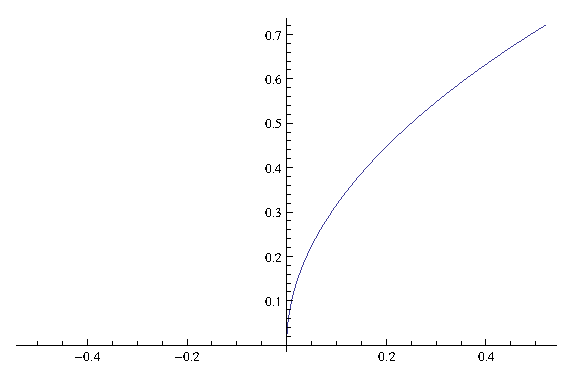
\includegraphics[width=0.3\textwidth]{continuous/functions/sqrtx}
    }
    \subfigure[A plot of $f^{-1}(\sqrt x)=x^2$.]{
      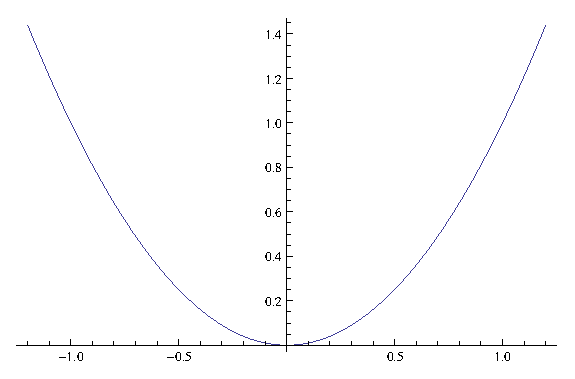
\includegraphics[width=0.3\textwidth]{continuous/functions/x2inv}
    }
  \end{center}
  \label{fig:inversef}
\end{figure}
\begin{remark} \index{composition}\index{inverse functions}
  By definition, either composite of a function and its inverse will return the identity function, where $y=x$. For example:
  \[ (f \circ f^{-1})(x)=f(f^{-1}(x))=x \]
  or
  \[ (f^{-1} \circ f)(x)=f^{-1}(f(x))=x. \]
\end{remark}

\subsection{Finding Inverse Functions}
To find the inverse of a function $f(x)$, replace $f(x)$ with $y$ and solve for $x$ in terms of $y$. Then, interchange $x$ and $y$.
\begin{ex}
  \label{ex:inverses}
  Find the inverse of $y=\frac{1}{2}x+1$, expressed as a function of $x$.
  \begin{sol}
    First, we solve the function for $x$ in terms of $y$.
    \begin{align*}
      y &= \frac{1}{2}x+1 \\
      \intertext{Multiply both sides by $2$.}
      2y &= x + 2 \\
      \intertext{Now subtract $2$ from both sides, and swap the left and right sides of the equation.}
      x &= 2y -2
      \intertext{Now we swap $x$ and $y$.}
      y &=2x-2
    \end{align*}
    The inverse of the function $f(x)=\frac{1}{2}x+1$ is the function $f^{-1}(x)=2x-2$.
    \begin{figure}[H]
      \begin{center}
        \subfigure[A plot of $f(x)=\frac{1}{2}x+1$.]{
          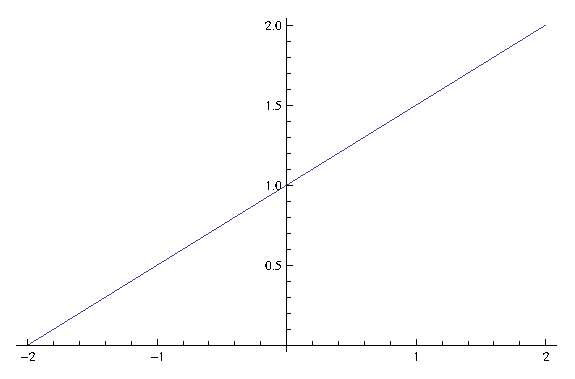
\includegraphics[width=0.45\textwidth]{continuous/functions/halfxeg}
        }
        \subfigure[A plot of $f^{-1}(x)=2x-2$.]{
          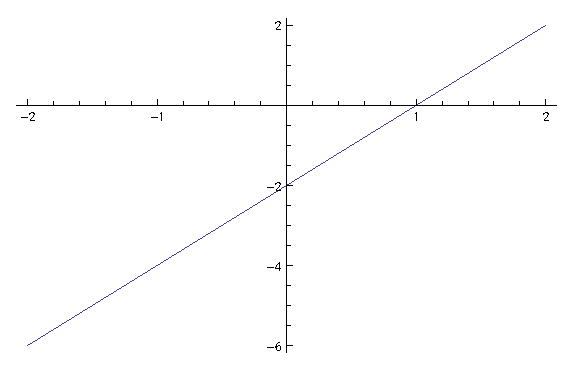
\includegraphics[width=0.45\textwidth]{continuous/functions/halfxeginv}
        }
      \end{center}
      \caption{Plots of functions from Example \ref{ex:inverses}.}
      \label{fig:inverseg}
    \end{figure}
  \end{sol}
\end{ex}

